\documentclass[10pt,aspectratio=169]{beamer}

\usetheme[progressbar=frametitle,sectionpage=none,background=light]{metropolis}

%%––––––––––––––––––––––––––––––––––––––––––––––––
% Define styles
%%––––––––––––––––––––––––––––––––––––––––––––––––

%%––––––––––––––––––––––––––––––––––––––––––––––––
% Setting up colors
\definecolor{logoblue1}{RGB}{35, 121, 181}
\definecolor{logoblue2}{RGB}{88, 145, 202}
\definecolor{darkblue}{RGB}{25, 41, 54}
\definecolor{lightgrey}{RGB}{134, 143, 161}
\definecolor{greytext}{RGB}{102, 118, 128}
\definecolor{darktext}{RGB}{29, 43, 52}
\definecolor{green}{RGB}{0, 184, 44}
\definecolor{vividblue}{RGB}{15, 117, 183}
\definecolor{orange}{RGB}{246, 177, 70}
\definecolor{lightblue}{RGB}{244, 247, 251}
\definecolor{white}{RGB}{255, 255, 255}
\definecolor{red}{RGB}{183, 25, 29}

\setbeamercolor{frametitle}{bg=darkblue, fg=lightblue}
\setbeamercolor{background canvas}{bg=black}
\setbeamercolor{normal text}{fg=lightblue}
%%––––––––––––––––––––––––––––––––––––––––––––––––

%%––––––––––––––––––––––––––––––––––––––––––––––––
% Setting up fonts
\usepackage{lato}
\usepackage{roboto}
\usepackage{montserrat}

\setbeamerfont{frametitle}{family=\flafamily, size*={18}{18}}
% \setbeamerfont{footline}{family=\fontfamily{montserrat}}
% \setbeamerfont{normal text}{family=\roboto, size*={16}{18}}

% Setting up fonts for bibliography style
\setbeamerfont{bibliography entry author}{size=\small}
\setbeamerfont{bibliography entry title}{size=\small}
\setbeamerfont{bibliography entry location}{size=\small}
\setbeamerfont{bibliography entry note}{size=\small}
\setbeamerfont{bibliography item}{size=\small}
%%––––––––––––––––––––––––––––––––––––––––––––––––

\usepackage{appendixnumberbeamer}

\usepackage{booktabs}
\usepackage[scale=2]{ccicons}

\usepackage{pgfplots}
\usepgfplotslibrary{dateplot}

\usepackage{xspace}
\newcommand{\themename}{\textbf{\textsc{metropolis}}\xspace}

\usepackage{hyperref}
\hypersetup{
  colorlinks, 
  urlcolor=vividblue, 
  citecolor=lightblue, 
  linkcolor=lightblue
}

\usepackage{graphicx}
\graphicspath{ {../imgs/} }

\usepackage{caption}

\title{\textcolor{orange}{Graph Embeddings}}
% \subtitle{A modern beamer theme}
\date{\today}
\author{Tim Semenov\\ \textcolor{vividblue}{timofei@sourced.tech}}
% \institute{Center for modern beamer themes}
%\titlegraphic{\hfill\includegraphics[height=1.5cm]{logo.png}}

\begin{document}

\maketitle

\setbeamertemplate{frame footer}{\large\textcolor{logoblue1}{source}\textcolor{logoblue2}{\{d\}}}

\begin{frame}{Table of contents}
  \setbeamertemplate{section in toc}[sections numbered]
  \tableofcontents[hideallsubsections]
\end{frame}


%%––––––––––––––––––––––––––––––––––––––––––––––––––––––––––––––––––––––––––––––––––––––––––––––––
\section{Introduction}

{
\usebackgroundtemplate{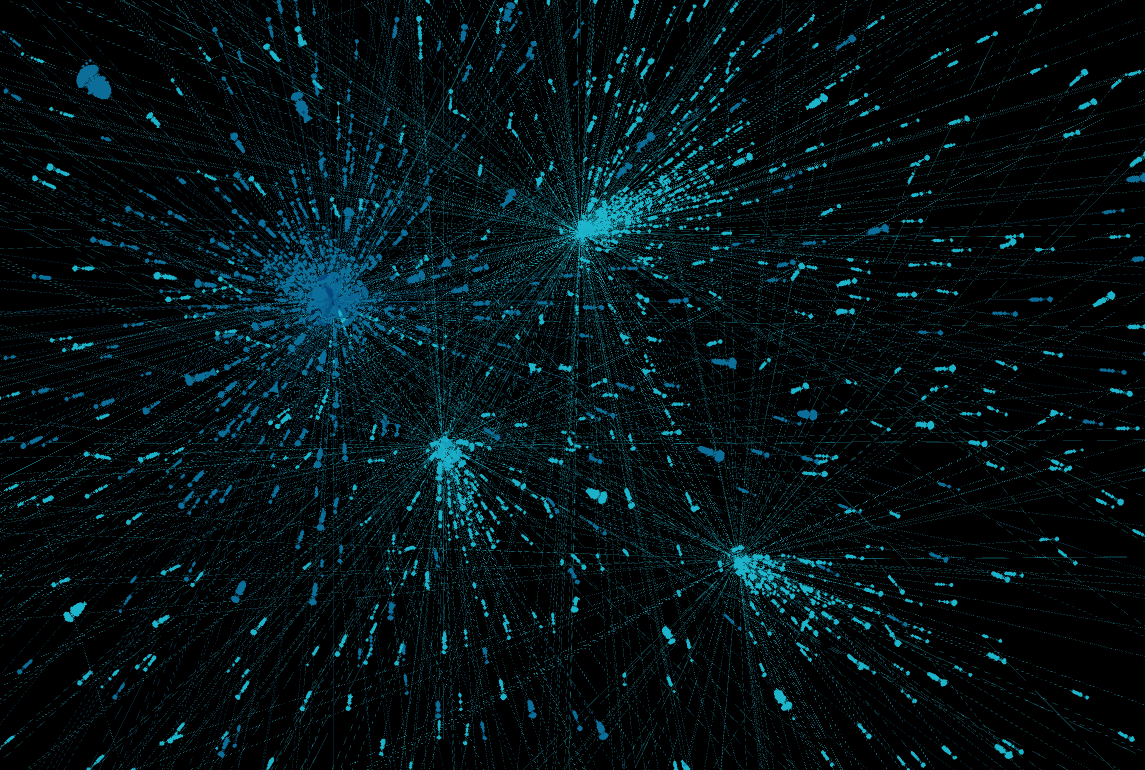
\includegraphics[width=\paperwidth]{img.png}}
\begin{frame}[fragile]{Introduction}
\end{frame}
}

\begin{frame}[fragile]{Notations}
  % A graph $G(V,E)$ is a collection of $V=\{v_1,\ldots,v_n\}$ vertices (a.k.a. nodes) and 
  % $E=\{e_{ij}\}^n_{i,j=1}$ edges. The adjacency matrix $S$ of graph $G$ contains non-negative
  % weights associated with each edge: $s_{ij}\geq0$. If $v_i$ and $v_j$ are not connected
  % to each other, then $s_{ij}=0$. For undirected weighted graphs, $s_{ij}=s_{ji} \hspace{1mm}
  % \forall \hspace{1mm} i,j \in [n]$.
  \begin{tabular}{ l l }
    Adjacency matrix: & $A$ \\
    Degree matrix: & $D=diag(\sum_j A_{ij})$ \\
    Transition matrix: & $M=D^{-1}A$\\
    Node neighborhood: & $N(i)$\\[4mm]
    \pause
    First-order proximity: & edges of adjacency matrix.\\
    Second-order proximity: & similarity between nodes' neighborhoods.
  \end{tabular}
\end{frame}

\begin{frame}[fragile]{Notations}
  Pointwise mutual information: $$PMI(x,y)=\log \frac{P(x,y)}{P(x)P(y)}$$
  Positive PMI: $$PPMI(x,y)=\max (PMI(x,y),0)$$
  Shifted PPMI: $$SPPMI_k(x,y)=\max (PMI(x,y)-\log k,0)$$
\end{frame}


%%––––––––––––––––––––––––––––––––––––––––––––––––––––––––––––––––––––––––––––––––––––––––––––––––
\section{Graph embeddings}

\begin{frame}[fragile]{Graph embedding methods}
  Taxonomy \cite{goyal2017graph}:
  \begin{enumerate}
    \item Factorization based
    \item Random Walk based
    \item Deep Learning based
    \item Other
  \end{enumerate}
\end{frame}

\begin{frame}[fragile]{Factorization}
  \begin{enumerate}
    \item HOPE \cite{ou2016asymmetric}
    \begin{itemize}
      \item $\displaystyle \min ||S-U^S{U^t}^T||_F^2$\\[1mm]
      \item $\displaystyle U=[U^S,U^t]$ -- the embedding matrix.\\[1mm]
      \item $S$ -- proximity matrix:
      \begin{itemize}
        \item[$\diamond$] $S=A^2 \;$ -- common neighbors.
        \item[$\diamond$] $S=ADA \;$ -- Adamic-Adar.
        \item[$\diamond$] \ldots
      \end{itemize}
    \end{itemize}

    \item GraRep \cite{Cao:2015:GLG:2806416.2806512}
    \begin{itemize}
      \item $X_k=SPPMI_{\beta}(A^k), \, k=1,\ldots,K$\\[1mm]
      \item $[U_k,\Sigma_k,V_k^T]=SVD(X_k)$\\[1mm]
      \item $W_k=U_{k,d}(\Sigma_{k,d})^{\frac{1}{2}}$
    \end{itemize}
  \end{enumerate}
\end{frame}

\begin{frame}[fragile]{Random Walk: node2vec}
  Optimization problem \cite{grover2016node2vec}: $$\max \sum_{v_i \in V} \log P(N(i)|v_i)$$
  Conditional independence: $$P(N(i)|v_i)=\prod_{j\in N(i)} P(v_j|v_i), \quad
    P(v_j|v_i)=\frac{\exp(u_j^{T}u_i)}{\sum_{k=1}^{|V|} \exp(u_k^{T}u_i)}$$
  \pause
  Simplified optimization problem: $$\max \sum_{v_i \in V} \Big[ -\log{Z_{v_i}} +
    \sum_{j \in N(i)} u_j^Tu_i \Big], \quad Z_{v_i}=\sum_{v_i \in V} \exp(u_j^Tu_i)$$
\end{frame}

\begin{frame}[fragile]{Random Walk: node2vec}
  Let $c_i$ denote the \textit{i}-th node in the random walk: $$P(c_i=x|c_{i-1}=v)=
    \begin{cases}
      \frac{\pi_{vx}}{Z} & \text{if } (v,x) \in E \\
      0 & \text{otherwise}
    \end{cases}$$
  Assume the walk just traversed edge $(t,v)$:
    $$\pi_{vx}=\alpha_{pq}(t,x)\cdot w_{vx}, \quad \alpha_{pq}(t,x)=
    \begin{cases}
      \frac{1}{p} & \text{if } d_{tx}=0\\
      1 & \text{if } d_{tx}=1\\
      \frac{1}{q} & \text{if } d_{tx}=2\\
    \end{cases}$$
\end{frame}

\begin{frame}[fragile]{Other: LINE}
  Joint probability between vertices \cite{2015arXiv150303578T}:
    $$P(v_i,v_j)=\frac{1}{1+\exp(-u_i^Tu_j)}, \quad \hat{P}(v_i,v_j)=\frac{w_{ij}}{W}$$
  Conditional distribution of the contexts:
    $$P(v_j|v_i)=\frac{\exp(u_j^{'T}u_i)}{\sum_{k=1}^{|V|} \exp(u_k^{'T}u_i)}, \quad \hat{P}(v_j,v_i)=\frac{w_{ij}}{d_i}$$
  \pause
  First-order proximity loss: $$O_1=-\sum_{(i,j)\in E} w_{ij} \log p_1(v_i,v_j)$$\\[2mm]
  Second-order proximity loss: $$O_2=-\sum_{(i,j)\in E} w_{ij} \log p_2(v_j|v_i)$$
\end{frame}

\begin{frame}[fragile]{Other: LINE}
  Use negative sampling to optimize $O_2$:
    $$\log \sigma(u_j^{'T}u_i)+\sum_{i=1}^K E_{v_n \sim P_n(v)}[\log \sigma(-u_n^{'T}u_i)]$$
  $O_1$ has a trivial minima, so we modify it to utilize negative sampling:
    $$\log \sigma(u_j^Tu_i)+\sum_{i=1}^K E_{v_n \sim P_n(v)}[\log \sigma(-u_n^{'T}u_i)]$$
  \pause
  In case of low degree we add weight to second-order neighbors:
    $$w_{ij}=\sum_{k \in N(i)} w_{ik} \frac{w_{kj}}{d_k}$$
\end{frame}

\begin{frame}[fragile]{Deep Learning: SDNE}
  Encoder-decoder model \cite{wang2016structural}:
    $$y_i^{(k)}=\sigma(W^{(k)}y_i^{(k-1)}+b^{(k)}), \; k=1,\ldots,K, \; y_i^{(0)}=x_i$$
    $$\hat{y}_i^{(k)}=\sigma(\hat{W}^{(k)}\hat{y}_i^{(k-1)}+\hat{b}^{(k)}), \; k=1,\ldots,K,
    \; \hat{y}_i^{(0)}=y_i^{(K)}, \; \hat{y}_i^{(K)}=\hat{x}_i$$
  \pause
  Loss functions:
    $$L_1=\sum_{i,j=1}^n a_{i,j} ||y_i^{(k)}-y_j^{(k)}||_2^2$$
    \pause
    $$L_2=\sum_{i=1}^n ||(\hat{x}_i-x_i) \odot b_i||_2^2, \quad b_{i,j}= 
    \begin{cases}
      1 & \text{if } a_{i,j}=0\\
      \beta > 1
    \end{cases}$$
    \pause
    $$L=L_2+\alpha L_1 + \nu L_{reg}, \quad L_{reg}=\frac{1}{2}\sum_{k=1}^K(||W^{(k)}||^2_F+||\hat{W}^{(k)}||^2_F)$$
\end{frame}


%%––––––––––––––––––––––––––––––––––––––––––––––––––––––––––––––––––––––––––––––––––––––––––––––––
\section{Experiment results}

\begin{frame}[fragile]{Datasets}
  \begin{itemize}
    \item \textcolor{orange}{Blogcatalog, Flickr and Youtube}\\
      Social networks of online users. Each user is labelled by at least one category.
    \item \textcolor{orange}{Arxiv GR-QC}\\
      Paper collaboration network which covers papers in the field of General Relativity 
      and Quantum Cosmology from arXiv.
    \item \textcolor{orange}{20-Newsgroup}\\
      Tf-idf vectors of each word are used to represent documents. The documents are 
      connected based on their cosine similarity.
  \end{itemize}
\end{frame}

\begin{frame}[fragile]{Datasets}
  \begin{table}
    \begin{tabular}{ccc}
      Dataset & |V| & |E|\\
      \textcolor{orange}{Blogcatalog} & 10312 & 667966\\
      \textcolor{orange}{Flickr} & 80513 & 11799764\\
      \textcolor{orange}{Youtube} & 1138499 & 5980886\\
      \textcolor{orange}{Arxiv GR-QC} & 5242 & 28980\\
      \textcolor{orange}{20-Newsgroup} & 1720 & Full-connected
    \end{tabular}
  \end{table}
\end{frame}

\begin{frame}[fragile]{Experiment: reconstruction task}
  \begin{table}
    \caption*{Arxiv GR-QC \cite{wang2016structural}}
    \begin{tabular}{ccccc}
      \hfill & SDNE & GraRep & LINE & DeepWalk\\
      MAP & \textcolor{orange}{0.836} & 0.05 & 0.69 & 0.58
    \end{tabular}
  \end{table}

  \begin{table}
    \caption*{Blogcatalog \cite{wang2016structural}}
    \begin{tabular}{ccccc}
      \hfill & SDNE & GraRep & LINE & DeepWalk\\
      MAP & \textcolor{orange}{0.63} & 0.42 & 0.58 & 0.28
    \end{tabular}
  \end{table}
\end{frame}

\begin{frame}[fragile]{Experiment: link prediction}
  \begin{table}
    \caption*{Arxiv GR-QC \cite{wang2016structural}}
    \begin{tabular}{cccccc}
      Algorithm & P@2 & P@10 & P@100 & P@200 & P@300\\
      SDNE & \textcolor{orange}{1} & \textcolor{orange}{1} & \textcolor{orange}{1} & \textcolor{orange}{1} & \textcolor{orange}{1}\\
      LINE & 1 & 1 & 1 & 1 & 0.99\\
      DeepWalk & 1 & 0.8 & 0.6 & 0.555 & 0.443\\
      GraRep & 1 & 0.2 & 0.04 & 0.035 & 0.033
    \end{tabular}
  \end{table}
\end{frame}


%%––––––––––––––––––––––––––––––––––––––––––––––––––––––––––––––––––––––––––––––––––––––––––––––––
\section{Conclusion}

\begin{frame}{Summary}
  \begin{itemize}
    \pause
    \item Use matrix factorization when you can.
    \pause
    \item Use random walk when matrix size is too large.
    \pause
    \item Use deeper models on top of rough embeddings.
  \end{itemize}
  \vspace{2mm}
  \pause
  Follow us on github:
  \begin{center}\url{https://github.com/src-d/role2vec}\end{center}
\end{frame}

\appendix

\begin{frame}[allowframebreaks]{References}

  \setbeamertemplate{bibliography item}{\insertbiblabel}
  \bibliography{references.bib}
  \bibliographystyle{abbrv}

\end{frame}

\end{document}
